\documentclass[portrait,color=UCLburgundy,margin=2cm]{uclposter}

\newcommand{\boldf}{\bm{f}}
\newcommand{\boldmu}{\bm{\mu}}
\newcommand{\boldalpha}{\bm{\alpha}}
\newcommand{\boldr}{\bm{r}}
\newcommand{\boldt}{\bm{t}}
\newcommand{\boldg}{\bm{g}}
\newcommand{\boldtheta}{\bm{\theta}}

% Warping operators
\newcommand{\MPWarp}{\tilde{\mathcal{W}}}
\newcommand{\Warp}{\mathcal{W}}

% Others
\newcommand{\etal}{\textit{et al.}~}
\newcommand{\ie}{i.e., }
\newcommand{\eg}{e.g., }

\usepackage{bm}
\usepackage{algorithm}
\usepackage{algorithmic}

\usepackage[acronym]{glossaries}
\newacronym{mu map}{mu map}{Attenuation Map}
\newacronym{TOF}{TOF}{Time Of Flight}
\newacronym{NAC}{NAC}{Non Attenuation Corrected}
\newacronym{RCM}{RCM}{Respiratory Correspondence Model}
\newacronym{MAPE}{MAPE}{Mean Absolute Percentage Error}
\newacronym{COM}{COM}{Centre Of Mass}
\newacronym{SIRF}{SIRF}{Synergistic Image Reconstruction Framework}
\newacronym{AP}{AP}{Anterior Posterior}
\newacronym{IS}{IS}{Inferior Superior}

\usepackage[style=ieee,maxbibnames=1,minbibnames=1,maxcitenames=1,mincitenames=1,backend=biber,defernumbers=false]{biblatex}
\addbibresource{./Biblio.bib}

\usepackage{fontspec}
\setmainfont[Ligatures=TeX]{LexendDeca-Regular.ttf}

\begin{document}

\title{Impact of Time-of-Flight on Respiratory Motion\newline Modelling using Non-Attenuation-Corrected PET}

\author[1,2 *]{Alexander C. Whitehead}
\author[1]{Elise C. Emond}
\author[3]{Nikos Efthimiou}
\author[1,2]{Adeyemi Akintonde}
\author[1]{Brian F. Hutton}
\author[2]{\newline Jamie McClelland}
\author[1]{Kris Thielemans}

\affil[1]{INM, University College London, UK}
\affil[2]{CMIC, University College London, UK}
\affil[3]{PET Research Centre, University of Hull, UK}
\affil[*]{alexander.whitehead.18@ucl.ac.uk}

\maketitle

\linespread{1.1}

\begin{multicols}{2}
\large

\section*{Introduction}
\begin{highlightbox}[UCLlightgreen]
    \begin{itemize}
        \item Respiratory motion causes artefacts and loss of resolution in PET. Surrogate driven motion models attempt to overcome these deficiencies by relating the motion in the data to a surrogate signal \cite{McClelland2013}.
        \item If images are reconstructed using a static \gls{mu map}, then artefacts caused by the misalignment between the activity distribution and the \gls{mu map} would hamper image registration.
        \item The aim of this work is to investigate whether \gls{TOF} information can sufficiently increase the contrast and lower the noise of \gls{NAC} images to facilitate the fitting of accurate motion models.
    \end{itemize}
\end{highlightbox}

\vspace{-2.0cm}

\section*{Methods}
\begin{itemize}

    \vspace{1.0cm}
    
    \subsection*{\underline{\textbf{Simulation}}}
    
    \vspace{-1.0cm}
    
    \item XCAT was used to generate volumes, the field of view included the lungs and diaphragm and a 40mm diameter spherical lesion placed in the right lung.
    \item  Acquisitions were simulated using STIR \cite{Efthimiou2018} through SIRF using the geometry of a GE Discovery 710 and a \gls{TOF} resolution of 375ps, similar to the GE Signa.
    \item Attenuation was included in the simulation. Scatter and randoms were not taken into account.
    \item  Acquisitions were simulated as if they had been gated into 6 bins over an acquisition of 120s.
    
    \subsection*{\underline{\textbf{Reconstruction}}}
    \item Data were reconstructed without attenuation correction using OSEM with 24 subsets and 2 full iterations and were post processed using a Gaussian blurring with a kernel size of 6.4mm.
    
    \subsection*{\underline{\textbf{Motion Estimation}}}
    \item NiftyRegResp \cite{McClelland2013} was used to estimate the \gls{RCM} which fits the motion estimated from the volumes to a surrogate signal representing the breathing motion.
    \item A direct correspondence motion model was used where the B spline coefficients at time $t$ are expressed as a linear combination of the 2 components of the surrogate, $s_{1,t}$ and $s_{2,t}$ , the \gls{AP} and \gls{IS} motion:
\end{itemize}
    
\begin{center}
    \resizebox{1\hsize}{!}
    {
        $\forall t \in [[1,n_t]], \quad \alpha_{k,t} := R_{1,k} s_{1,t} + R_{2,k} s_{2,t} + R_{3,k}$
    }
\end{center}
    
\noindent where $\alpha_{k,t}$ is the 3D B-spline coefficient for node $k$ at time point $t$, and $R_{i,k}$ are the model parameters.
    
\begin{highlightbox}[UCLlightgreen]
    \subsection*{\underline{\textbf{Evaluation}}}
    3 \gls{RCM}s were compared, calculated from the XCAT volumes, non-\gls{TOF} \gls{NAC} and \gls{TOF} \gls{NAC} reconstructions. These were used to warp a reference volume. The estimated volumes were then compared to the original XCAT volumes.
\end{highlightbox}

\vspace{-2.0cm}

\section*{Results}
\begin{table}[H]
  \centering
  
  \begin{highlightbox}[UCLlightblue]
      \caption{Comparison of the \gls{MAPE} between the ground truth data and the volumes estimated from the XCAT, the \gls{NAC} non-\gls{TOF} and the \gls{NAC} \gls{TOF} based \gls{RCM}.}
  \end{highlightbox}
  
  \vspace{2.0cm}
  
  \resizebox{0.5\linewidth}{!}
  {
    \begin{tabular}{||c|ccc||}
      \hline
        \textbf{\gls{MAPE}} & \textbf{XCAT} & \textbf{non-\gls{TOF}} & \textbf{\gls{TOF}} \\
      \hline
        \textbf{1} & 1.95 & 8.35 & 4.18 \\
        \textbf{2} & 1.59 & 1.61 & 1.84 \\
        \textbf{3} & 2.06 & 9.91 & 5.23 \\
        \textbf{4} & 1.97 & 6.15 & 3.68 \\
        \textbf{5} & 1.65 & 4.45 & 2.52 \\
        \textbf{6} & 1.95 & 8.35 & 4.18 \\
      \hline
        \textbf{Mean} & 1.86 & 6.47 & 3.60 \\
      \hline
    \end{tabular}
  }
  \label{tab:MAPE}
\end{table}

\begin{figure}[H]
  \centering
  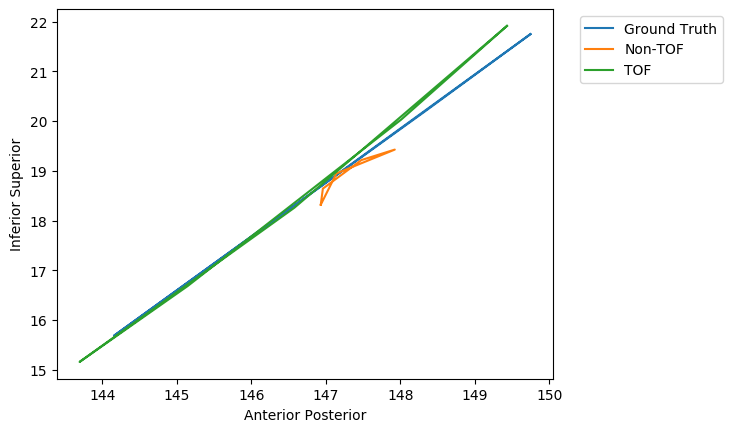
\includegraphics[width=0.8\linewidth]{TOF.png}
  \begin{highlightbox}[UCLlightblue]
      \caption{The path of the \gls{COM} of the lesion. Different curves denote \gls{COM} for ground truth, XCAT, \gls{NAC} non-\gls{TOF} and \gls{NAC} \gls{TOF} based \gls{RCM} estimated data}
  \end{highlightbox}
  \label{fig:com_graph}
\end{figure}

\end{multicols}

\begin{figure*}[h!]
  \centering
  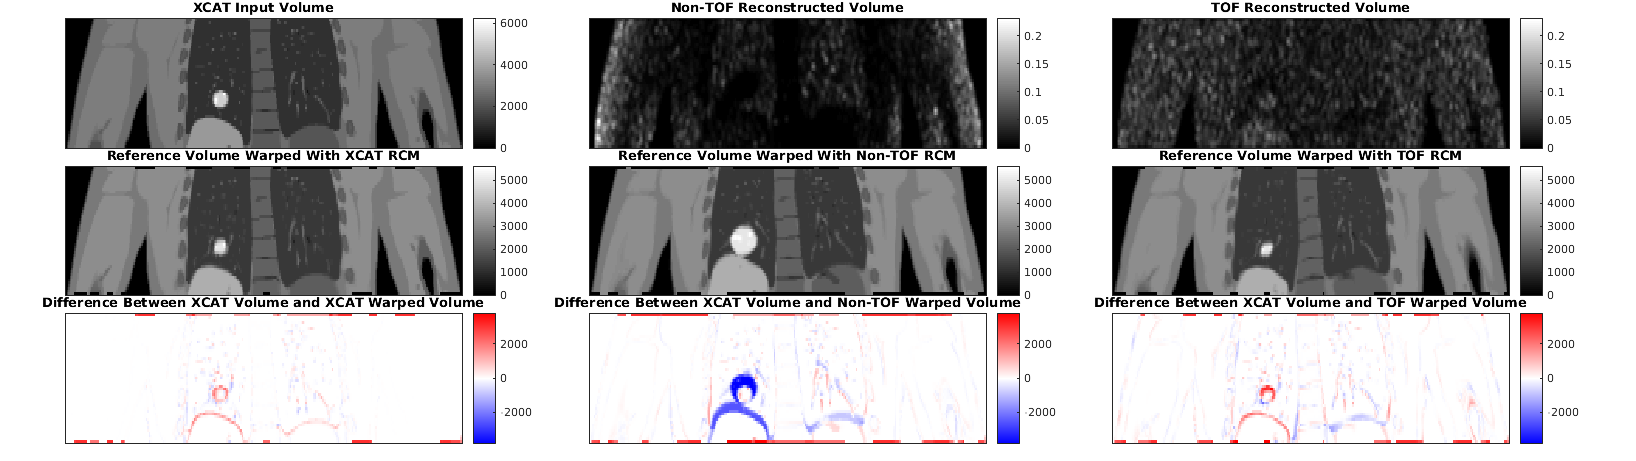
\includegraphics[width=1\linewidth]{output.png}
  
  \begin{highlightbox}[UCLlightblue]
      \caption{All volumes correspond to end inhalation. First row from left to right: XCAT PET, NAC non-TOF and NAC TOF reconstructed data. Second row: RCM applied to reference position XCAT data with RCM derived from XCAT PET data (left), NAC non-TOF (middle) and NAC TOF (right) volumes. The third row: The difference between the estimated volumes from the second row with the XCAT end inhalation volume.}
  \end{highlightbox}
  
  \label{fig:output}
\end{figure*}

\begin{multicols}{2}

\AtNextBibliography{\footnotesize}
\printbibliography

\footnotesize
\section*{Acknowledgements}
This research is supported by GE Healthcare, the NIHR UCLH Biomedical Research Centre and the EPSRC funded UCL Centre for Doctoral Training in Medical Imaging (EP/L016478/1).
Elise C. Emond is supported by GlaxoSmithKline (BIDS3000030921).

\end{multicols}

\end{document}
